\documentclass[11pt, a4paper]{article}
\usepackage[slovak]{babel}
\usepackage[utf8]{inputenc}

\usepackage{graphicx}
\usepackage{indentfirst}
\usepackage{cite}

\author{Peter Schmiedt, Eduard Füzesséry}
\title{Lékařská informatika - Úloha zpracování a analýzy dat}

\graphicspath{{fig/}{logo/}}

\begin{document}

\begin{titlepage}
	\maketitle
\end{titlepage}



\section{Úvod}
Cieľom tejto úlohy je spracovanie a analýza dát z testovania účinnosti liečby dvoch rôznych liekov na primárnu chorobu a aký majú na to vplyv vek, BMI, sekundárne choroby, prítomnosť inej medikácie, atď.


Ďalšou úlohou je nájsť zaujímavé fakty a náväznosti medzi veličinami štatistickej významnosti.

\section{Spracovávané Dáta}



\begin{figure}[h!]
	\centering
  		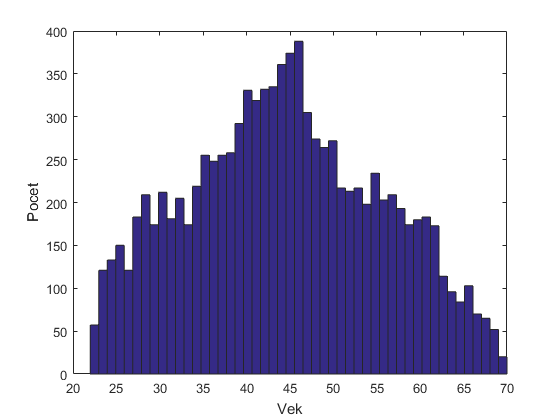
\includegraphics[width=1.0\textwidth]{ages.png}
  	\caption{Histogram Vekov}
\end{figure}

\bibliography{literatura}{}
\bibliographystyle{plain}

\end{document}
